\chapter{Teoria dei residui}

Nel momento in cui lo sviluppo in serie di Laurent presenta una singolarità isolata, abbiamo una naturale classificazione delle singolarità.\\Ma procediamo per gradi: innanzitutto, diamo la definizione di singolarità isolata:
\begin{definizione}
Un punto $a \in \C$ è una \textbf{singolarità isolata} per la funzione $f$ se $f$ è olomorfa nel disco forato $D'(a,r)=D(a,r) \backslash \{a\}$ per un valore di $r>0$.
\end{definizione}
Una volta trovato sìffatto disco, possiamo scrivere lo sviluppo in serie di Laurent, ottenendo come già visto:
$$\sum_{n=-\infty} ^{+\infty} c_n (z-a)^n=\sum_{n=0} ^{+\infty} c_n (z-a)^n + \sum_{n=1} ^{+\infty} c_{-n} \frac{1}{(z-a)^n}$$
Possiamo osservare come la parte principale diverga per $z \to a$; a seconda di come è fatta la parte principale, classifichiamo le singolarità isolate nella seguente maniera:
\begin{itemize} 
\item La singolarità si dice \textbf{rimovibile} se i coefficienti $c_{-n}$ sono  nulli $\forall n \geq 1$ (cioè se la parte principale è nulla). Un esempio è la funzione $\frac{sen(z)}{z}$; infatti sviluppandola in $z=0$ otteniamo:
$$\frac{sen(z)}{z}= \frac{1}{z} \left(z-\frac{z^3}{3!} + \frac{z^5}{5!}+ \dots \right)=1-\frac{z^2}{3!} + \frac{z^4}{5!}+ \dots$$
cioè lo sviluppo non ha parte principale.
\item La singolarità si dice \textbf{polo di ordine n} se i coefficienti $c_{-n}$ sono definitivamente nulli, cioè se $c_{-n} \neq 0$ e $c_{-n-k}=0$ $\forall k \geq 1$. \\
Un esempio è la funzione $f(z)=\frac{1}{(z-3)^3}$, che coincide con il suo sviluppo in serie di Laurent centrato in $z=3$ e che risulta avere in tale punto un polo di ordine 3.
\item  La singolarità si dice \textbf{essenziale} se, diversamente dal polo di ordine n, i coefficienti della parte principale non sono definitivamente nulli, cioè se $\forall N>0$ $\exists k>N$ : $c_{-k} \neq 0$. \\ Un esempio è la funzione $f(z)=e^{\frac{1}{z}}$, il cui sviluppo di Laurent centrato in $z=0$ è:
$$\sum_{n=0} ^{\infty} \frac{1}{n!} \frac{1}{z^n}$$
cioè lo sviluppo ha solo parte principale.
\end{itemize}
%Nel caso di singolarità essenziale, non è definito il limite di $f(z)$ per $z \to a$; nel caso di polo di ordine n, tale limite è infinito; invece, nel caso di singolarità essenziale abbiamo che
\begin{definizione}
Una funzione si dice \textbf{meromorfa} su un domnio $\mathbb{D}$ se è olomorfa su $\mathbb{D}$ a meno di un insieme di singolarità isolate.
\end{definizione}
Concentriamoci ora sulla parte principale dello sviluppo in serie di Laurent di una funzione $f(x)$ con singolarità in $z=a$. Il coefficiente $c_{-1}$ dello sviluppo centrato in $z=0$ è detto \textbf{residuo} di $f$ in $z=a$ e si indica come:
$$c_{-1}=Res[f,a]=\oint_{\gamma} \frac{dz}{2 \pi i} f(z)$$
dove l'ultima uguaglianza e data dalla definizione dei coefficienti $c_n$ dello sviluppo di Laurent.
\\
Proviamo ad esempio a calcolare il residuo della funzione $f(z)=\frac{1}{z(z-1)}$, che presenta un polo semplice nei punti $z=0$ e $z=1$; abbiamo che:
\begin{itemize}
\item Nel disco forato $0<|z|<1$:
$$f(z)=\frac{1}{z} (-1) \sum_{n=0} ^{\infty} z^n = -\frac{1}{z} -1 -z-z^2- \dots$$
cioè $Res[f,0]=-1$.
\item Se invece scegliamo l'anello $|z|>1$:
$$f(z)= \frac{1}{z^2(1-\frac{1}{z})} = \frac{1}{z^2} \left[1+\frac {1}{z}+\frac{1}{z^2}+\dots \right]=\frac {1}{z^2}+\frac{1}{z^3}+\dots$$
cioè in questo caso si ha che $Res[f,0]=0$, poichè la singolarità non è essenziale; quindi, per poter classificare la singolarità, dobbiamo trovarci nel disco forato nel quale abbiamo tolto solo tale singolarità.
\end{itemize}

\section{Calcolo dei residui}
$$Res[f,a]=c_{-1}=\oint_{\gamma} \frac{dz}{2 \pi i} f(z)$$
A seconda del tipo di singolarità, il residuo ha valori diversi:
\begin{itemize}
\item Nel caso in cui la singolarità sia rimovibile, abbiamo che
$$Res[f,a]=0$$
\item Nel caso in cui la singolarità sia un polo semplice, lo sviluppo di Laurent centrato in $z=a$ é del tipo $f(z)=\frac{c_{-1}}{z-a}+c_0+c_1(z-a)+c_2(z-a)^2+ \dots$; quindi abbiamo che il coefficiente $c_{-1}$ può essere visto come:
$$c_{-1}=\lim_{z\to a} (z-a) f(z)$$
\item Nel caso in cui la singolarità sia un polo di ordine n, abbiamo che lo sviluppo di Laurent centrato in $z=a$ è del tipo:
$$f(z)=\frac{c_{-n}}{(z-a)^n}+ \dots + \frac{c_{-1}}{z-a}+c_0+c_1(z-a)+ \dots$$
Moltiplicando per $(z-a)^n$ otteniamo:
$$(z-a)^nf(z)=c_{-n}+ c_{n-1}+ \dots + c_{-1}(z-a)^{n-1}+c_0 (z-a)^n\dots$$
e si vede che, derivando ($n-1$)-volte l'espressione, eliminiamo tutti i coefficienti di ordine $k<-1$; oltretutto, dividiamo per $(n-1)!$, in modo tale che il coefficiente $c_{-1}$ rimanga isolato. Otteniamo dunque che:
$$\frac{1}{(n-1)!} \frac{d^{n-1}}{dz^{n-1}} [(z-a)^k f(z)]=c_{-1}+k c_0(z-a)+ \dots$$
e, passando al limite per $z \to a$, abbiamo il valore del residuo:
$$c_{-1}= \lim_{z \to a} \frac{1}{(n-1)!} \frac{d^{n-1}}{dz^{n-1}} [(z-a)^k f(z)]$$
\item Se la singolarità è essenziale, a meno di casi particolari, dobbiamo sempre ricondurci alla definizione dei coefficienti $c_{-1}$, cioè dobbiamo calcolarci $\oint_{\gamma} \frac{dz}{2 \pi i} f(z)$. \\Ad esempio, per calcolare il $Res[z^3 e^{\frac{1}{z}},0]$, dobbiamo calcolare $\oint_{\gamma} \frac{dz}{2 \pi i} z^3 e^{\frac{1}{z}}$; questo esempio è anche uno dei casi particolari in cui possiamo fare a meno di ricorrere alla definizione dei coefficienti della serie di Laurent: infatti, abbiamo che lo sviluppo di $z^3 e^{\frac{1}{z}}$ è:
$$f(z)=z^3 \sum_{n=0} ^{\infty} \frac{1}{k!} \frac{1}{z^k}=z^3+\frac{z^2}{2!}+\frac{z}{3!} +\frac{1}{4!} +\frac{1}{5!} \frac{1}{z} +\dots$$
cioè si ha che $Res[z^3 e^{\frac{1}{z}},0]=c_{-1}=\frac{1}{5!}$.
\end{itemize}
%Alcuni esempi
\begin{teorema} (Teorema dei Residui) \\
Sia $f$ una funzione olomorfa su un dominio $\mathbb{D} \backslash \mathcal{S}$, dove $\mathcal{S}$ è un'insieme di singolarità isolate di $f$ nel dominio $\mathbb{D}$; sia poi $\gamma$ un cammino chiuso contenuto in $\mathbb{D} \backslash \mathcal{S}$ tale che
$$Ind[\gamma,z]=0 \text{ se il punto } z \notin \mathbb{D}$$
Allora si ha che
$$\oint_{\gamma} f(z) dz = 2 \pi i \sum_{z_k \in \mathcal{S}} Res[f,z_k]\, Ind[\gamma,z_k]$$
\end{teorema}
Essenzialmente questo teorema ci permette di calcolare il valore di un integrale come somma dei residui di $f$ sulle sue singolarità, ma solo per quelle contenute nel dominio (da qui la richiesta che $Ind[\gamma,z]=0$ per i punti $z \notin \mathbb{D}$).
\\
\\
Vediamo ora la dimostrazione:
\begin{proof}
Per ogni singolarità isolata esiste un disco forato nel quale vale uno sviluppo di Laurent della forma:
$$f(z)=P_k(z)+A_k(z)$$
dove $P_k(z)$ e $A_k(z)$ sono dei polinomi che rappresentano rispettivamente la parte principale e la parte analitica dello sviluppo.\\
Costruiamo ora la funzione ausiliaria $g$ definita come:
$$g(z)=f(z)- \sum_k P_k(z)$$
Dimostriamo che questa funzione è olomorfa in $\mathbb{D}$. Per il teorema di Cauchy, si ha che $\oint_{\gamma} g(z)dz=0$; ma per definizione di $g$, abbiamo che $\oint_{\gamma} g(z)dz=\oint_{\gamma} f(z)dz - \sum_k \oint_{\gamma} P_k(z) dz$. \\
Per definizione, sappiamo che il termine $\oint_{\gamma} P_k(z) dz$ varrà $2 \pi i \, c_{-1} ^{(k)} Ind[\gamma,z_k]$ poichè , dato che la curva $\gamma$ non tocca nessuna singolarità, tutti i termini $\frac{c_{-n} ^{(k)}}{(z-z_k)^n}$ (con $n>1$) ammettono primitiva, e quindi il loro integrale su un cammino chiuso è nullo. Otteniamo quindi la tesi.

\end{proof}

Sia data la funzione $f(x)=\frac{1}{x^4+1}$; per calcolare l'integrale della funzione su tutto l'asse reale, ricorriamo al teorema dei residui; infatti, possiamo passare al campo complesso scrivendo:
$$\int_{-\infty} ^{+\infty} \frac{dx}{x^4+1}= \lim_{R \to \infty} \int_{-R} ^{+R} \frac{dx}{x^4+1}=\lim_{R \to \infty} \oint_{\gamma} \frac{dz}{z^4+1}$$
dove la curva $\gamma$ è quella rappresentata in figura sotto; si nota che l'ultimo passaggio è lecito perchè l'integrale sulla semicirconferenza si annulla per $R \to \infty$.
\begin{figure}[h!]
  \centering
    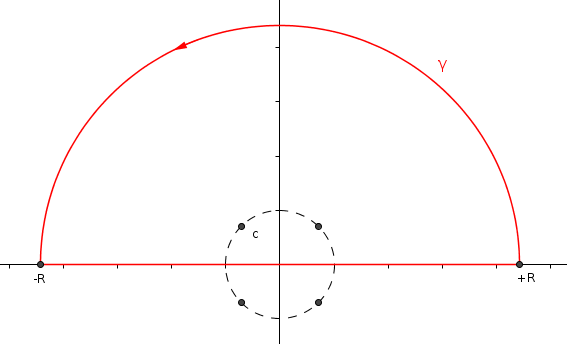
\includegraphics[width=0.5\textwidth]{immagini/esempio_residui.png}
\end{figure}
La funzione $f$ presenta quattro singolarità; esse sono tutti poli semplici e si trovano tutti sulla circonferenza unitaria.
Applicando quindi il teorema dei residui, abbiamo che:
$$ \oint_{\gamma} \frac{dz}{z^4+1}= 2 \pi i \left( Res \left[ \frac{1}{z^4+1}, e^{i \frac{\pi}{4}} \right] + Res \left[ \frac{1}{z^4+1}, e^{i \frac{3 \pi}{4}} \right] \right)$$
Calcoliamo i due residui separatamente:
$$Res \left[ \frac{1}{z^4+1}, e^{i \frac{\pi}{4}} \right]= \lim_{z \to e^{i \frac{\pi}{4}}} (z- e^{i \frac{\pi}{4}}) \frac{1}{z^4+1}=\footnote{Si ricorda che possiamo riscrivere $z^4+1$ come $(z-e^{i \frac{\pi}{4}})(z-e^{i \frac{3 \pi}{4}})(z-e^{i \frac{5 \pi}{4}})(z-e^{i \frac{7 \pi}{4}})$.}\lim_{z \to e^{i \frac{\pi}{4}}} \frac{1}{(z-e^{i \frac{3 \pi}{4}})(z-e^{i \frac{5 \pi}{4}})(z-e^{i \frac{7 \pi}{4}})}=$$
$$=\frac{1}{(e^{i \frac{\pi}{4}}-e^{i \frac{3 \pi}{4}})(e^{i \frac{\pi}{4}}-e^{i \frac{5 \pi}{4}})(e^{i \frac{\pi}{4}}-e^{i \frac{7 \pi}{4}})}=\frac{1}{e^{i \frac{3 \pi}{4}}} \frac{1}{(1-e^{i \frac{\pi}{2}})(1- e^{i \pi})(1- e^{i \frac{3 \pi}{2}})}=\frac{e^{-i \frac{3 \pi}{4}}}{(1-i)(2)(1+i)}=\frac{e^{-i \frac{3 \pi}{4}}}{4}$$
Allo stesso modo, calcoliamo $Res \left[\frac{1}{z^4+1}, e^{i \frac{3 \pi}{4}} \right]$, ottenendo:
$$Res\left[\frac{1}{z^4+1}, e^{i \frac{3 \pi}{4}} \right]= \dots =-\frac{e^{i \frac{3 \pi}{4}}}{4}$$
Adesso, risostituendo nella formula iniziale, otteniamo:
$$ \oint_{\gamma} \frac{dz}{z^4+1}= 2 \pi i \left(Res \left[ \frac{1}{z^4+1}, e^{i \frac{\pi}{4}} \right] + Res \left[ \frac{1}{z^4+1}, e^{i \frac{3 \pi}{4}} \right] \right)=2 \pi i \left(\frac{e^{-i \frac{3 \pi}{4}}}{4} -\frac{e^{i \frac{3 \pi}{4}}}{4} \right)=$$
$$=2 \pi i \left(\frac{1}{2} \frac{e^{-i \frac{3 \pi}{4}} - e^{i \frac{3 \pi}{4}}}{2} \right)=2 \pi i \left(\frac{1}{2} \left(-i \right) sen \left(\frac{3 \pi}{4} \right) \right)= \frac{\pi}{\sqrt{2}}$$
Quindi abbiamo ricavato il valore dell'integrale iniziale, cioè:
$$\int_{-\infty} ^{+\infty} \frac{dx}{x^4+1}=\frac{\pi}{\sqrt{2}}$$

\section{Gli integrali trigonometrici}

Il teorema dei residui può essere sfruttato per valutare degli integrali altrimenti di non facile determinazione, i cosìddetti \textbf{integrali trigonometrici}.
\\
\\
Calcoliamo ad esempio il valore di
$$\int_0 ^{2 \pi} \frac{cos(4 \theta)}{2+ cos \theta}d \theta$$
Abbiamo diversi metodi per calcolare tale integrale: possiamo sfruttarele proprietà trigonometriche per scrivere:
$$\int_0 ^{2 \pi} \frac{e^{i 4 \theta}+e^{-i 4 \theta}}{4+ e^{i \theta} + e^{-i \theta}}d \theta$$
ed effettuando un cambio di variabili:
$$\oint_{|z|=1} \frac{z^4 + \frac{1}{z^4}}{4+z+\frac{1}{z}} \frac{dz}{iz} = \oint_{|z|=1} \frac{z^4 + \frac{1}{z^4}}{4z+z^2+1} \frac{dz}{i}$$
Però in questo caso risulta ''scomodo'' il calcolo del polo di ordine 4.\\
Un'altra stradapossibile dopo aver ridotto l'integrale trigonometrico ad un integrale complesso è quella di porre prima $z=e^{i \theta}$ e poi $z=e^{-i \theta}$, cioè percorrere la circonferenza di raggio unitario prima in senso antiorario, poi in senso orario.
\\
\\
Possiamo aggirare i problemi derivanti dai precedenti due metodi considerando $Re[\int_0 ^{2 \pi} \frac{e^{i 4 \theta}}{2+ cos \theta}d \theta]$, che è ovviamente una riscrittura dell'integrale di partenza. Ponendo $z=e^{i \theta}$, l'integrale risulta:
$$\int_0 ^{2 \pi} \frac{cos(4 \theta)}{2+ cos \theta}d \theta=Re \left[\int_0 ^{2 \pi} \frac{e^{i 4 \theta}}{2+ cos \theta}d \theta \right]= Re \left[ \oint_{|z|=1} \frac{z^4}{2+\frac{z+\frac{1}{z}}{2}} \frac{dz}{iz} \right]=$$
$$=2Re \left[\oint_{|z|=1} \frac{z^4}{z^2+4z+1} \frac {dz}{i} \right]=\footnote{Gli zeri del denominatore sono $z_{1,2}=\frac{-4 \pm \sqrt{16-4}}{2}=-2 \pm \sqrt{3}$. Osseriviamo che solo $z_1$ si trova all'interno della circonferenza di raggio 1.} 2Re \left[\oint_{|z|=1} \frac{z^4}{(z-z_1)(z-z_2)} \frac {dz}{i} \right]=$$
$$=2Re \left[\frac{2 \pi i}{i}  \lim_{z \to z_1} (z-z_1) \frac{z^4}{(z-z_1)(z-z_2)} \right]=\frac{4 \pi z_1 ^4}{z_1-z_2}=4 \pi \frac{(\sqrt{3}-2)^4}{2 \sqrt{3}}$$
\\
\\
Quando viene richiesto di calcolare un'integrale su tutto l'asse reale, per poter passare agli integrali complessi (e quindi sfruttare il teorema dei residui) dobbiamo scegliere un cammino chiuso che sia equivalente a quello di partenza, cioè per il quale il contributo della ''linea di raccordo'' fra il semiasse positivo e il semiasse negativo (nel limite di $R \to \infty$) sia nullo. I percorsi che vengono solitamente scelti per comodità sono:
\begin{figure}[h!]
  \centering
    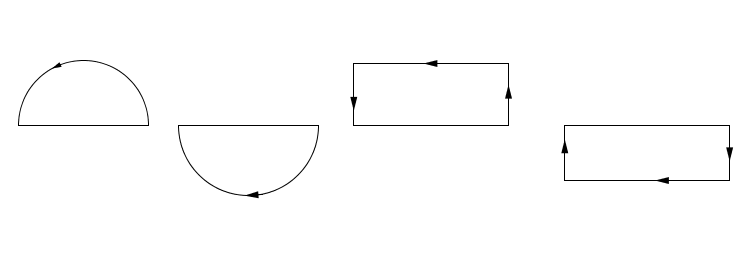
\includegraphics[width=0.8\textwidth]{immagini/percorsi_possibili.png}
\end{figure}
\\
Ad esempio per calcolare il valore dell'integrale $\int_{-\infty} ^{+\infty} dx f(x) \frac{e^{-ikz}}{\sqrt{2 \pi}}$ (la trasformata di Fourier della funzione $f$) abbiamo che, a seconda dei valori di $k$, dobbiamo scegliere percorsi diversi:
\begin{itemize}
\item Se $k>0$ scegliamo la semicirconferenza inferiore
\item Se $k<0$ scegliamo la semicirconferenza superiore
\end{itemize}
Questo è dovuto alla struttura dei numeri complessi; infatti, posto $z=x+iy$, abbiamo che:
$$e^{-ikz}=e^{-ik(x+iy)}=e^{-ik} e^{ky}$$
e quindi, per le richieste di annullamento del contributo della semicirconferenza, abbiamo i risultati citati sopra.
%Altri esempi
\begin{lemma} (di Jordan)\\
Se il contributo del semicerchio si annulla a $+\infty$, allora tale contributo è nullo.
\end{lemma}
Vediamo che questo fatto si verifica. Prendiamo $\int_{\cap} dz f(z) e^{ikz}$, con $k>0$ e $f$ continua; definiamo poi $M(r)=\sup_{\theta \in [0,\pi]} |f(r e^{i \theta})|$, dove abbiamo parametrizzato la circonferenza come $z=r e^{i \theta}$. Applicando la parametrizzazione anche all'integrale e prendendone il modulo, otteniamo:
$$\left|\int_{\cap} dz f(z) e^{ikz}\right|=\left|\int_0 ^{\pi} ird\theta f(r e^{i \theta}) e^{ikr(cos \theta + i sen \theta)}\right| \leq r \int_0 ^{\pi} d \theta |f(r e^{i \theta})| e^{-kr \, sen\theta} \leq$$
$$\leq r M(r) \int_0 ^{\pi} d \theta e^{-kr \, sen\theta} = 2 r M(r) \int_0 ^{\frac{\pi}{2}} d \theta e^{-kr \, sen\theta} \leq$$
$$\leq 2 r M(r) \int_0 ^{\frac{\pi}{2}} d \theta e^{-\frac{2kr}{\pi} \theta}=2rM(r) \frac{1-e^{-kr}}{\frac{2kr}{\pi}} \leq \frac{\pi}{k} M(r)$$
\begin{osservazione}
Nell'utilizzare il Lemma di Jordan dobbiamo stare attenti al segno di k; infatti, non è detto che valga anche per $k \leq 0$.
\end{osservazione}
%Altri esempi





